\chapter{Die Natürliche Sprache}


Die \textbf{Verarbeitung natürlicher Sprache} (NLP) ist ein theoretisch motivierter Bereich von Computertechniken, zum Analysieren und Darstellen natürlich vorkommender Texte auf einer oder mehreren Ebenen der Sprachanalyse, um eine menschenähnliche Sprachverarbeitung für eine Reihe von Aufgaben oder Anwendungen zu erreichen \cite*{Liddy}.

Der Umgang mit Textdaten ist problematisch, da unsere Computer, Skripte und Modelle für maschinelles Lernen, keinen Text im menschlichen Sinne lesen und verstehen können. Wörter können viele verschiedene Assoziationen aufrufen, diese sprachlichen Assoziationen sind das Ergebnis recht komplexer neurologischer Berechnungen. ML-Modelle sind haben dieses vorgefertigte Verständnis der Wortbedeutung nicht.


% regular expressions
% tokenize
% part of speech tagging
% ngrams

\section{Tokenisieren und Extrahieren durch Reguläre Ausdrücke}
Das Segmentieren eines Textes in seine Einheiten ist die erste Voraussetzung für dessen Weiterverarbeitung. In der Informatik können einzelne Wörter bzw. Tokens durch Leerzeichen voneinander abgetrennt werden.

Reguläre Ausdrücke können die Tokenisierung verbessern. Reguläre Ausdrücke sind eine Sprache zur Angabe von Textsuchzeichenfolgen. Diese praktische Sprache wird in allen Computersprachen, Textverarbeitungs- und Textverarbeitungswerkzeugen verwendet. Formal ist ein regulärer Ausdruck eine algebraische Notation zur Charakterisierung einer Reihe von Zeichenfolgen. Sie sind besonders nützlich für die Suche in Texten, wenn ein Muster gesucht wird und ein Korpus von Texten durchsucht werden muss. Eine Suchfunktion für reguläre Ausdrücke durchsucht den Korpus und gibt alle Texte zurück, die dem Muster entsprechen. Der Korpus kann ein einzelnes Dokument oder eine Sammlung sein \cite*[3]{Jurafskya}. Reguläre Ausdrücke sind also bestimmte Regeln die Muster in einem Text erkennen lassen. Neben der Tokenisierung können sie auch für das extrahieren von Informationen aus Textsequenzen verwendet werden, siehe Listing~\ref{Regex}.


\begin{lstlisting}[language=Python,caption=Das extrahieren der Zahlen aus einer URL]
>>> import re
>>> url = "http://www.example.com/this-2-me-4/123456-subj"
>>> print(re.search("/([0-9]+)-", url).group(1))

123456
\end{lstlisting}\label{Regex}
\section{N-Gramm}

Sprachmodelle sind Wortfolgen zu denen Wahrscheinlichkeiten zugewiesen wurden. Das einfachste Sprachmodell ist das N-Gramm Sprachmodell. Es ist eine Folge von N Wörtern (ein 2-Gramm oder Bigramm ist eine Folge von zwei Wörtern usw.). N-Gramm wird meistens dafür verwendet, um das nächste Wort in aus einer Sequenz vorherzusagen \cite*[31]{Jurafskya}. Angenommen ein Korpus besteht aus folgenden 4 Sätzen:

\begin{enumerate}
    \item Es regnet in Berlin.
    \item Es regnet in Köln und es ist 10 Grad.
    \item Es regnet und hagelt in ganz Deutschland.
    \item In Deutschland herrscht Regen.
\end{enumerate}

Um die Wahrscheinlichkeit \textit{P (regnet | in)} herauszufinden, wird die Anzahl des Wortes \enquote{regnet} im Korpus gezählt. Es wird gezählt, wie oft \enquote{regnet} und \enquote{in} zusammen vorkommen (2 Mal) und dieses wird dividiert durch 3, da \enquote{regnet} insgesamt 3 Mal im Korpus vorkommt. Das Bigramm \enquote{regnet in} hat also eine Wahrscheinlichkeit von 2/3.

\section{Part-of-Speech Tagging}
Part-of-Speech Tagging ist der Prozess des Zuweisens einer Tags zu jedem Wort in einem Eingabetext. Die Eingabe in einen Kennzeichnungsalgorithmus ist eine Folge von tokenisierten Wörtern und einem Tag-Satz, und die Ausgabe ist eine Folge von Tags, eines pro Token \cite*[148]{Jurafskya}. Je nach Sprache gibt es verschiedene Tagger, für das Deutsche gibt es das Stuttgart-Tübingen-Tagset\cite*{tagger}, einige Tags können aus der Tabelle~\ref{STTS} entnommen werden. Die Tagger wurden ursprünglich manuell erfasst und in heutiger Zeit durch das Maschinelle Lernen automatisiert.



\begin{table}[h]
    \caption{Beispiele aus dem Stuttgart-Tübingen-Tagset}
    \label{STTS}
    \renewcommand{\arraystretch}{1.2}
    \centering
    \sffamily
    \begin{footnotesize}
        \begin{tabular}{l l l}
            \toprule
            \textbf{POS} & \textbf{Beschreibung}                  & \textbf{Beispiel}                                  \\
            \midrule
            ADJA         & attributives Adjektiv                  & das \textit{große} Haus                            \\
            ADJD         & adverbiales oder prädikatives Adjektiv & er fährt \textit{schnell}, er ist \textit{schnell} \\
            ADV          & Adverb                                 & \textit{schon}, \textit{bald}, doch                \\
            NE           & Eigennamen                             & \textit{Hans}, \textit{Hamburg}, \textit{HSV}      \\
            NN           & normales Nomen                         & \textit{Tisch}, \textit{Herr}, das \textit{Reisen} \\
            VVFIN        & finites Verb, voll                     & du \textit{gehst}, wir \textit{kommen} an          \\
            \bottomrule
        \end{tabular}
    \end{footnotesize}
    \rmfamily
\end{table}




\section{Wie können Deep Learning Modelle die Natürliche Sprache lernen?}

Die verborgenen Schichten eines mehrschichtigen neuronalen Netzwerks lernen, die Eingaben des Netzwerks so darzustellen, dass die Zielausgaben leicht vorhergesagt werden können. Dies wird gut demonstriert, indem ein mehrschichtiges neuronales Netzwerk trainiert wird, um das nächste Wort in einer Sequenz aus einem lokalen Kontext früherer Wörter vorherzusagen \cite*{Bengio2003}. Jedes Wort im Kontext wird dem Netzwerk als Eins-aus-N-Vektor dargestellt, dh eine Komponente hat den Wert 1 und der Rest ist 0, dieses Verfahren wird auch als \textit{One-Hot-Encoding} bezeichnet. In einem \textit{Sprachmodell} lernen die anderen Schichten des Netzwerks, die Eingangswortvektoren in einen Ausgangswortvektor für das vorhergesagte nächste Wort umzuwandeln, welches verwendet werden kann, um die Wahrscheinlichkeit vorherzusagen, dass ein Wort im Vokabular als nächstes erscheinen wird \cite*{Lecun2015}. Das Netzwerk lernt \textbf{Wortvektoren}, die viele aktive Komponenten enthalten, von denen jede als separates Merkmal des Wortes interpretiert werden kann. Dieses Vorgehen wurde erstmals im Zusammenhang mit dem Lernen verteilter Darstellungen für Symbole demonstriert \cite*{Rumelhart1986}. Die semantischen Merkmale waren in der Eingabe nicht explizit vorhanden. Das Lernverfahren wurde als eine gute Möglichkeit entdeckt, die strukturierten Beziehungen zwischen den Eingabe- und Ausgabesymbolen in mehrere \enquote{Mikroregeln} zu zerlegen. Das Lernen von Wortvektoren hat sich auch als sehr gut erwiesen, wenn die Wortsequenzen aus einem großen Korpus von echtem Text stammen und die einzelnen Mikroregeln unzuverlässig sind \cite*{Bengio2003}.


\begin{figure}[H]
    \centering
    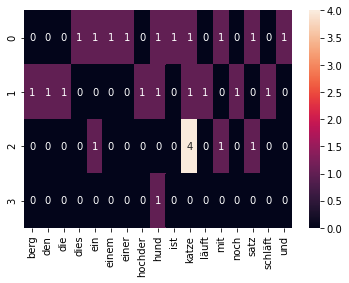
\includegraphics[width=8cm]{kapitel3/onhot.png}
    \caption[One-Hot-Codierung als Eingabematrix]{Die Grafik zeigt wie ein Beispielkorpus welches aus 5 Sätzen besteht, in einer Matrix dargestellt werden kann. Je nach Häufigkeit wird jedes Wort im Wortschaft entsprechend den Sätzen im Korpus abgebildet. Der Korpus besteht aus 5 Sätzen (\enquote{Dies ist ein Satz mit einer Katze und einem Hund.}, \enquote{Die Katze läuft den Berg hoch.}, \enquote{Der Hund schläft noch.}, \enquote{Ein Satz mit Katze Katze Katze Katze.} und \enquote{Ein Hund.}) (eigene Darstellung).}
    \label{OneHotGrafik}
\end{figure}

Die numerischen Werte sollten so viel wie möglich von der sprachlichen Bedeutung eines Wortes erfassen. Eine gut ausgewählte, informative Eingabedarstellung kann einen massiven Einfluss auf die Gesamtleistung des Modells haben. \textbf{Worteinbettungen} sind der vorherrschende Ansatz für dieses Problem und so weit verbreitet, dass ihre Verwendung praktisch in jedem NLP-Projekt angenommen wird. Unabhängig davon, ob Sie ein Projekt in den Bereichen Textklassifizierung, Sentimentanalyse oder maschinelle Übersetzung starten \cite*{Lecun2015}.


\section{Worteinbettungen}
Vektoren zur Darstellung von Wörtern werden im Allgemeinen als Einbettungen bezeichnet, da das Wort in einen bestimmten Vektorraum eingebettet wird \cite*[99]{Jurafskya}.

\begin{figure}[H]
    \centering
    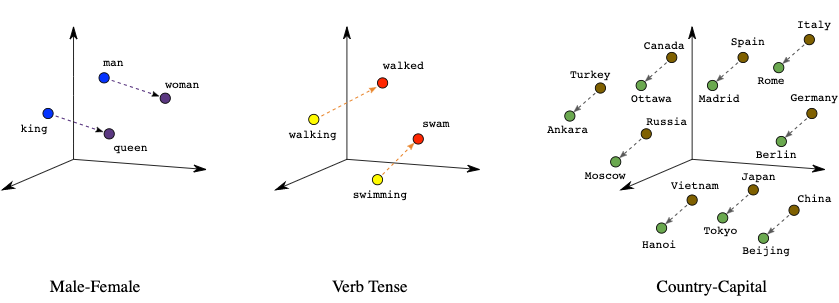
\includegraphics[width=14cm]{kapitel3/wordem.png}
    \caption[Worteinbettungen erzeugen Analogien zwischen Wörtern]{Durch Worteinbettungen können interessante Analogien zwischen einzelnen Wörtern gefunden werden. (Entnommen aus \cite*{wordemdgood})}
    \label{Word2Vex}
\end{figure}


\textbf{Word2Vec} \cite*{Mikolov2013} Worteinbettungen sind Vektordarstellungen von Wörtern, die normalerweise von einem Modell gelernt werden, wenn große Textmengen als Eingabe eingegeben werden (z. B. Wikipedia, Wissenschaft, Nachrichten, Artikel usw.). Diese Darstellung von Wörtern erfasst die semantische Ähnlichkeit zwischen Wörtern unter anderen Eigenschaften. Word2Vec-Worteinbettungen werden so gelernt, dass der Abstand zwischen Vektoren für Wörter mit enger Bedeutung (z. B. \enquote{König} und \enquote{Königin}) näher ist als der Abstand für Wörter mit völlig unterschiedlichen Bedeutungen (z. B. \enquote{König} und \enquote{Katze}).

Bei der \textit{One-Hot-Codierung} sind die Wörter \enquote{gut} und \enquote{großartig}  genauso unterschiedlich wie \enquote{Tag} und \enquote{Nacht}. Hier kommt die Idee, verteilte Darstellungen zu erzeugen. Intuitiv wird eine gewisse Abhängigkeit eines Wortes von den anderen Wörtern eingeführt. Die Wörter im Kontext dieses Wortes würden einen größeren Anteil dieser Abhängigkeit erhalten. In der One-Hot Darstellung dagegen, sind alle Wörter unabhängig voneinander.



\section{Word2Vec mit der Skip-Gram Architektur}

Wörter können als spärliche, lange Vektoren mit vielen Dimensionen dargestellt werden. Eine alternative Methode ist die Darstellung eines Wortes mit der Verwendung von \textit{kurzen Vektoren}, mit einer Länge von 50-1000 und einer \textit{großen dichte} (die meisten Werte sind nicht Null). Es stellt sich heraus, dass dichte Vektoren in jeder NLP-Aufgabe besser funktionieren als spärliche Vektoren. Erstens können dichte Vektoren erfolgreicher als Features in maschinellen Lernsystemen aufgenommen werden.

Wenn beispielsweise 100-dimensionale Worteinbettungen als Merkmale verwendet werden, kann ein Klassifikator nur 100 Gewichte lernen, um die Bedeutung des Wortes darzustellen. Wenn  stattdessen einen 50.000-dimensionalen Vektor eingeben wird, müsste ein Klassifikator Zehntausende von Gewichten für jede der spärlichen Dimensionen lernen. Zweitens können dichte Vektoren besser verallgemeinern und helfen, eine Überanpassung zu vermeiden, da sie weniger Parameter als spärliche Vektoren mit expliziten Zählungen enthalten. Schließlich können dichte Vektoren die Synonyme besser erfassen als spärliche Vektoren. Zum Beispiel sind \textit{Auto} und \textit{Automobil} Synonyme. In einer typischen spärlichen Vektordarstellung sind beide Dimensionen unterschiedliche Dimensionen. Da die Beziehung zwischen diesen beiden Dimensionen nicht modelliert wird, können spärliche Vektoren möglicherweise die Ähnlichkeit zwischen Auto und Automobil als Nachbarn nicht erfassen \cite*[110-111]{Jurafskya}.


\begin{figure}[H]
    \centering
    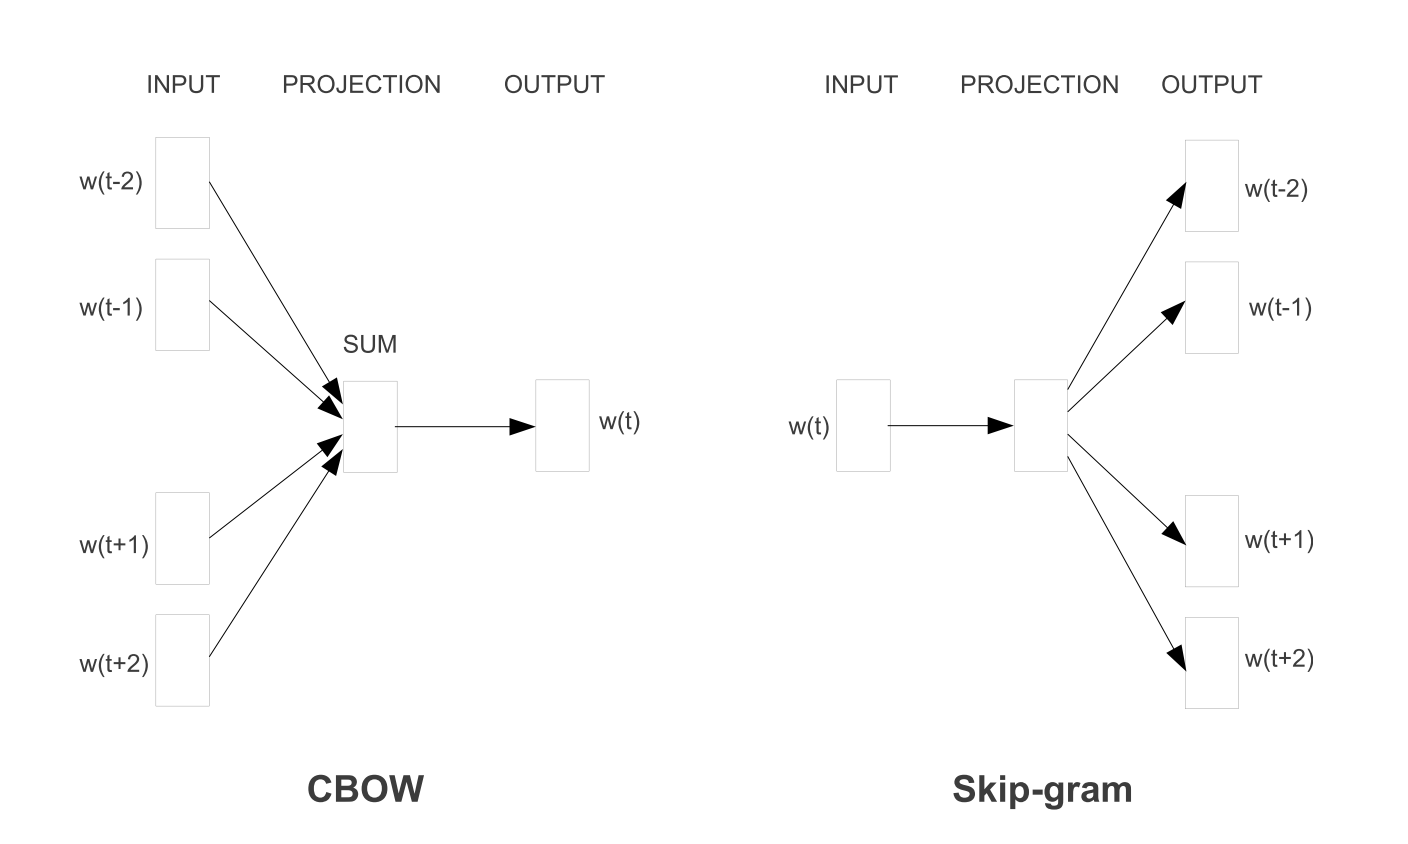
\includegraphics[width=12cm]{kapitel3/cbowskipgr.png}
    \caption[Vergleich zwischen CBOW und Skip-Gram Architektur]{Die CBOW-Architektur sagt das aktuelle Wort basierend auf dem Kontext voraus, während das Skip-Gramm die umgebenden Wörter voraussagt, wenn das aktuelle Wort gegeben ist aus \cite*{Mikolov}).}
    \label{cbowskipgr}
\end{figure}

Der Skip-Gram-Algorithmus ist einer von zwei Algorithmen in einem Softwarepaket namens \textbf{word2vec} \cite*{Mikolov2013}\cite*{Mikolov}. Die Intuition von word2vec ist, dass anstatt zu zählen, wie of jedes Wort $w$ in der Nähe von einem anderen Wort vorkommt, einen Klassifikator für eine binäre Vorhersageaufgabe zu trainieren. Die erlernten Klassifikatorgewichte werden dann als Worteinbettungen genommen \cite*[111]{Jurafskya}. Dabei wird ein Zielwort $t$ mit Kandidaten aus dem Kontext \textit{c} in ein \textit{Tupel} gesetzt. \textit{P(+|t,c)} sagt dann aus, wie wahrscheinlich es ist, dass ein Kontextwort \textit{c} ein echter Kontext ist. Zum Beispiel sei gegeben der Satz \enquote{Wir essen Spaghetti zum Abendessen...}. Wenn der Kontext von $\pm 2$ Wörter betrachtet wird, und \textit{t} das Zielwort \enquote{essen} ist, wird die Klassifikation für das Tupel \textit{(essen,spaghetti)} \enquote{true} und für das Tupel \textit{(essen,auto)} \enquote{false} zurückgeben \cite*[111]{Jurafskya}.

\begin{equation} \label{Formel3_1}
    P(-|t,c) = 1-P(+|t,c)
\end{equation}

Die Ähnlichkeit eines Wortes zu einem anderen Wort, kann mittels Skalarprodukt berechnet werden. Dies ist zunächst nur eine Zahl zwischen $-\infty$ und $+\infty$. Um daraus eine Wahrscheinlichkeit zu berechnen, wird die \textit{sigmoid} Funktion $\sigma(x)$ angewendet. Die Logistikfunktion gibt eine Zahl zwischen 0 und 1 zurück. Um die Wahrscheinlichkeit zu berechnen, muss gewährleistet werden, dass die Summe \textit{c ist das Kontextwort} und \textit{c ist nicht das Kontextwort} eine 1 ergeben \cite*[112]{Jurafskya}.

\begin{equation} \label{Formel3_2}
    P(-|t,c) = 1-P(+|t,c) = \frac{e^{-t\cdot c}}{1+e^{-t\cdot c}}
\end{equation}

Skip-Gramm macht die starke, aber sehr nützliche vereinfachende Annahme, dass alle Kontextwörter unabhängig sind, so dass ihre Wahrscheinlichkeiten multipliziert werden können:

\begin{equation} \label{Formel3_3}
    P(+|t,c_{1:k}) = \prod ^{k}_{i=1}\frac{1}{1+e^{-t\cdot c_{i}}}
\end{equation}

\begin{equation} \label{Formel3_4}
    \log P(+|t,c_{1:k}) =\sum ^{k}_{i=1} \log \frac{1}{1+e^{-t\cdot c_{i}}}.
\end{equation}


Word2vec lernt Einbettungen, indem es mit einem anfänglichen Satz von Einbettungsvektoren beginnt und dann die Einbettung jedes Wortes $w$ iterativ verschiebt, um mehr in der Nähre der Einbettungen von Wörtern zu kömmen die ähneln. Für das Training eines binären Klassifikators werden negative Beispiele nötig. Das Skip-Gram benötigt mehr negative als positive Beispiele für das Training. Das Verhältnis zwischen positiven und negativen Beispielen wird mit einem Parameter $k$ festgelegt. Für jedes der Trainingseinheiten \textit{t, c} werden \textit{k} negative Stichproben erstellt, die jeweils aus dem Ziel \textit{t} und einem \enquote{noise word} besteht. Ein \enquote{noise word} is ein zufälliges Wort aus dem Lexikon, das nicht das Zielwort \enquote{t} sein darf \cite*[113]{Jurafskya}.

Das Ziel des Lernalgorithmus besteht darin, mittels gegebenen positiven und negativen Beispielen diese Einbettungen so anzupassen, dass die Ähnlichkeit der Ziel- und Kontextwortpaare \textit{(t, c)} aus den positiven Beispielen maximiert werden und die Ähnlichkeit der Paare \textit{(t, c)} aus den negativen Beispielen minimiert wird. Formell lässt sich dieses mit folgender Formel ausdrücken:

\begin{gather} \label{Formel3_5}
    L(\theta) = \sum_{(t,c)\in +}\log P(+|t,c)+\sum_{(t,c)\in -} \log P(-|t,c) =  \notag\\
    \log \sigma(c \cdot t)+\sum^{k}_{i=1}\log \sigma(-n_{i} \cdot t) = \notag\\
    \log \frac{1}{1+e^{-c \cdot t}}+\sum^{k}_{i=1}\log\frac{1}{1+e^{n_{1} \cdot t}}.
\end{gather}

Die stochastische Gradientenabstieg kann verwendet werden, um dieses Ziel zu erreichen, indem die Parameter (die Einbettungen für jedes Zielwort $t$ und jedes Kontextwort oder \enquote{noise word} $c$ im Vokabular) iterativ modifiziert werden \cite*[114]{Jurafskya}.


\section{CNN in der Textverarbeitung}
Anstelle von Bildpixeln können die Eingaben für die meisten NLP-Aufgaben Sätze oder Dokumente, als eine Matrix dargestellt werden. Jede Zeile der Matrix entspricht einem Token, normalerweise einem Wort, aber es kann sich auch um ein Zeichen handeln. Das heißt, jede Zeile ist ein Vektor, der ein Wort darstellt. Typischerweise sind diese Vektoren Worteinbettungen (niedrigdimensionale Darstellungen) wie word2vec oder GloVe, aber sie können auch One-Hot-Vektoren sein, die das Wort in ein Vokabular indizieren. Für einen 10-Wort-Satz unter Verwendung einer 100-dimensionalen Einbettung hätten wir eine 10 × 100-Matrix als Eingabe \cite*{Zhang}.

In der Vision \enquote{gleiten} die Filter über lokale \enquote{pathces} eines Bildes, in NLP wird jedoch der Filter über die ganze Zeilen der Matrix (Wörter) gleiten. Daher entspricht die Breite der Filter normalerweise der Breite der Eingabematrix. Die Höhe oder Regionsgröße kann variieren, aber \enquote{Schiebefenster} mit jeweils mehr als 2-5 Wörtern sind typisch. Pixel, die nahe beieinander liegen, sind wahrscheinlich semantisch verwandt (Teil desselben Objekts), aber das Gleiche gilt nicht immer für Wörter. In vielen Sprachen können Teile von Phrasen durch mehrere andere Wörter getrennt werden. Der kompositorische Aspekt ist ebenfalls nicht offensichtlich. Es ist klar, dass Wörter in gewisser Weise zusammengesetzt sind, wie ein Adjektiv, das ein Substantiv modifiziert, aber wie genau dies funktioniert, was Darstellungen auf höherer Ebene tatsächlich \enquote{bedeuten}, ist nicht so offensichtlich wie im Fall von Computer Vision. Angesichts all dessen scheinen CNNs nicht gut für NLP-Aufgaben geeignet zu sein. Wiederkehrende neuronale Netze (RNNs) sind intuitiver. Sie ähneln der Art und Weise, wie wir Sprache verarbeiten (oder zumindest wie wir denken, dass wir Sprache verarbeiten). Lesen nacheinander von links nach rechts. Glücklicherweise bedeutet dies nicht, dass CNNs nicht funktionieren. Alle Modelle sind falsch, aber einige sind nützlich. Es stellt sich heraus, dass CNNs, die auf NLP-Probleme angewendet werden, recht gut funktionieren. Ein großes Argument für CNNs ist, dass sie schnell sind. Faltungen sind ein zentraler Bestandteil der Computergrafik und werden auf Hardwareebene auf GPUs implementiert. Mit einem großen Wortschatz kann das Berechnen schnell \enquote{teuer} werden. Faltungsfilter lernen automatisch gute Darstellungen, ohne das gesamte Vokabular darstellen zu müssen \cite*{widlml}.

\begin{figure}[H]
    \centering
    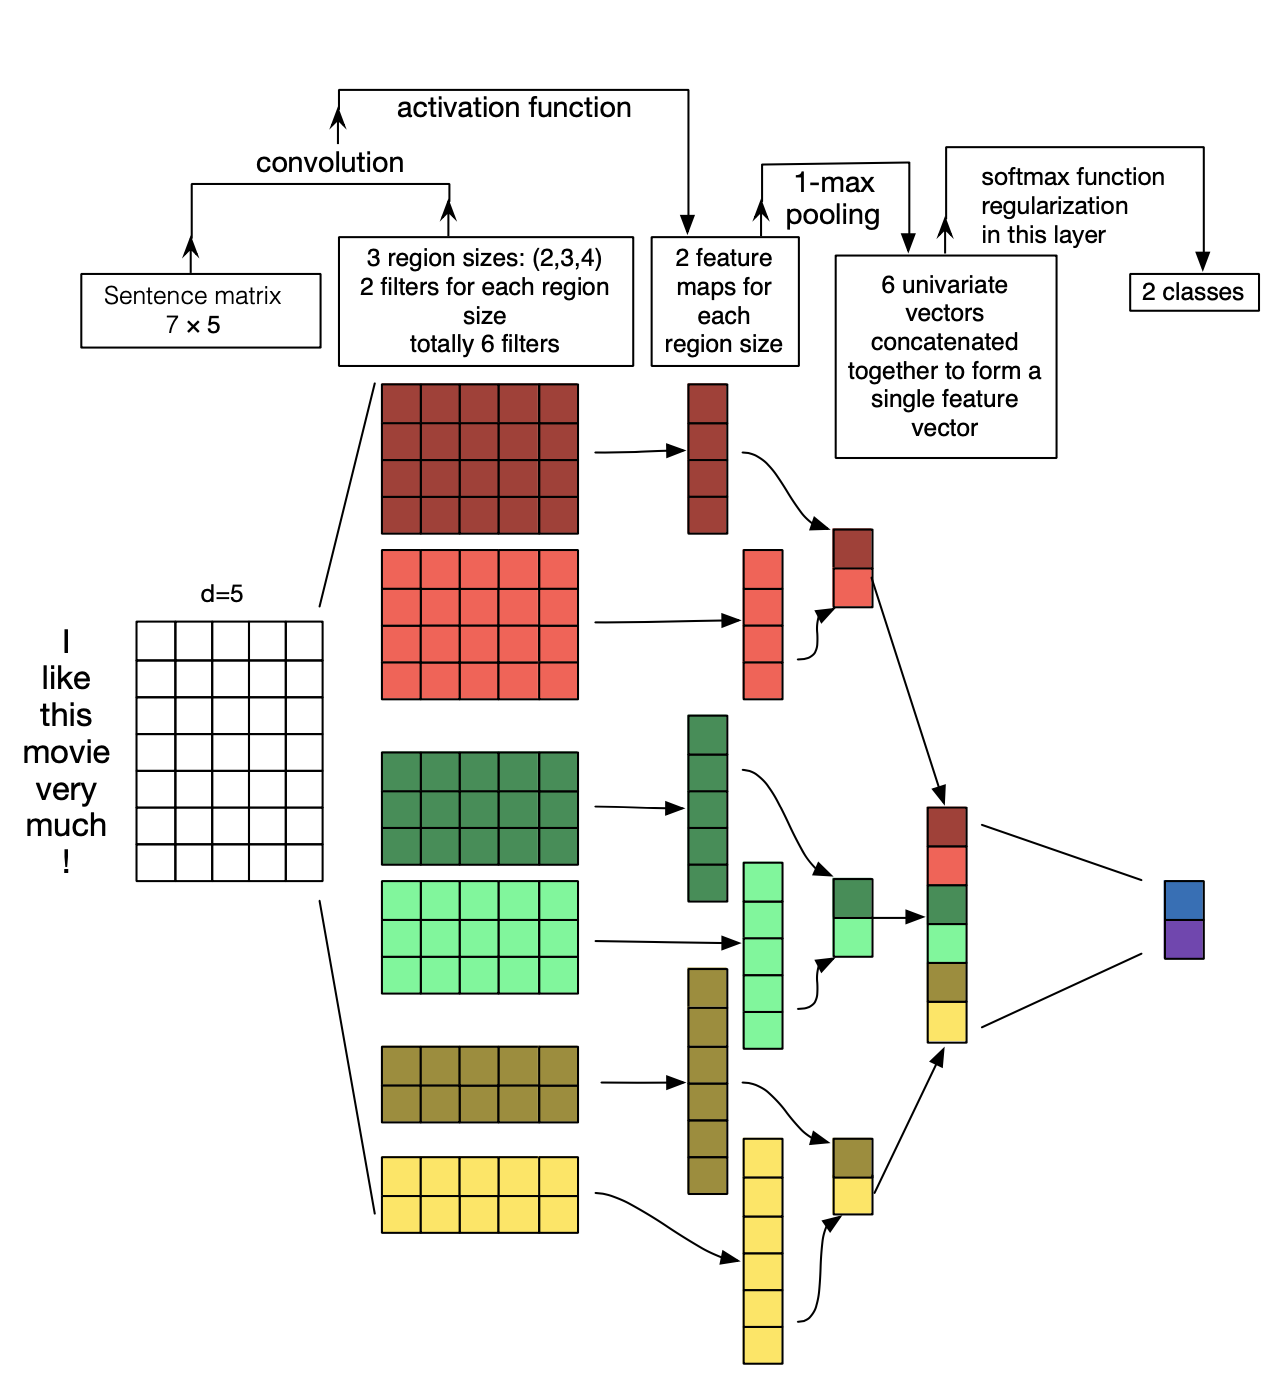
\includegraphics[width=10cm]{kapitel2/cnnnlp.png}
    \caption[CNN in der Textverarbeitung]{Illustration einer CNN-Architektur zur Satzklassifizierung. Es sind drei Filterbereichsgrößen vorhanden: 2, 3 und 4. Filter führen Faltungen in der Satzmatrix durch und generieren Feature-Maps (mit variabler Länge). Über jede Karte wird ein 1-Max-Pooling durchgeführt, d. H. die größte Anzahl von jeder Merkmalskarte wird aufgezeichnet. Somit wird aus allen sechs Karten ein univariater Merkmalsvektor erzeugt, und diese sechs Merkmale werden verkettet, um einen Merkmalsvektor für die vorletzte Schicht zu bilden. Die letzte Softmax-Schicht empfängt dann diesen Merkmalsvektor als Eingabe und verwendet ihn zur Klassifizierung des Satzes an. Hier wird eineeine binäre Klassifikation angewendet und es gibt daher zwei mögliche Ausgangszustände dar \cite*{Zhang}.}
    \label{Kap2:Pooling}
\end{figure}

% \subsubsection{Glove}
% Eine andere Methode zum Einbetten von Wörtern ist Glove (\enquote{Global Vectors}). Es basiert auf Matrixfaktorisierungstechniken für die Wortkontextmatrix. Zunächst wird eine große Matrix von Informationen zum gleichzeitigen Auftreten von Wörter und Kontext erstellt, d. H. für jedes \enquote{Wort} (die Zeilen) wird gezählt, wie häufig dieses Wort in einem \enquote{Kontext} (den Spalten) in einem großen Korpus angezeigt wird. Dann wird diese Matrix in eine niederdimensionale Matrix Wort und Merkmale zerlegt, in der jede Zeile nun eine Vektordarstellung für jedes Wort speichert. Dies geschieht im Allgemeinen durch Minimierung eines \enquote{Rekonstruktionsverlusts}. Dieser Verlust versucht, die niederdimensionalen Darstellungen zu finden, die den größten Teil der Varianz in den hochdimensionalen Daten erklären können.




% \chapter{Grobe Zeit- und Ressourcenplanung}
% % \label{Kap3}
% Grobe Zeitplanung und die Anteile der Kapitel and er Arbeit:
% \begin{itemize}
%     \item \textbf{November 2020 bis Oktober 2020:} Kapitel 2, 3 (ca. 25\%)
%     \item \textbf{Dezember 2020} Kapitel 4-5 (ca. 25\%)
%     \item \textbf{Januar 2021:} Kapitel 6 (ca. 20\%)
%     \item \textbf{Februar 2021:} Kapitel 7 (ca. 20\%)
%     \item \textbf{März 2021:} Kapitel 1, 8 (ca. 10\%)
% \end{itemize}
% \section{Bilder}

% Natürlich können auch Grafiken und Bilder eingebunden werden, siehe z.\,B. Abbildung~\ref{Kap2:NasaRover}.

% \begin{figure}[ht]
%     \centering
%     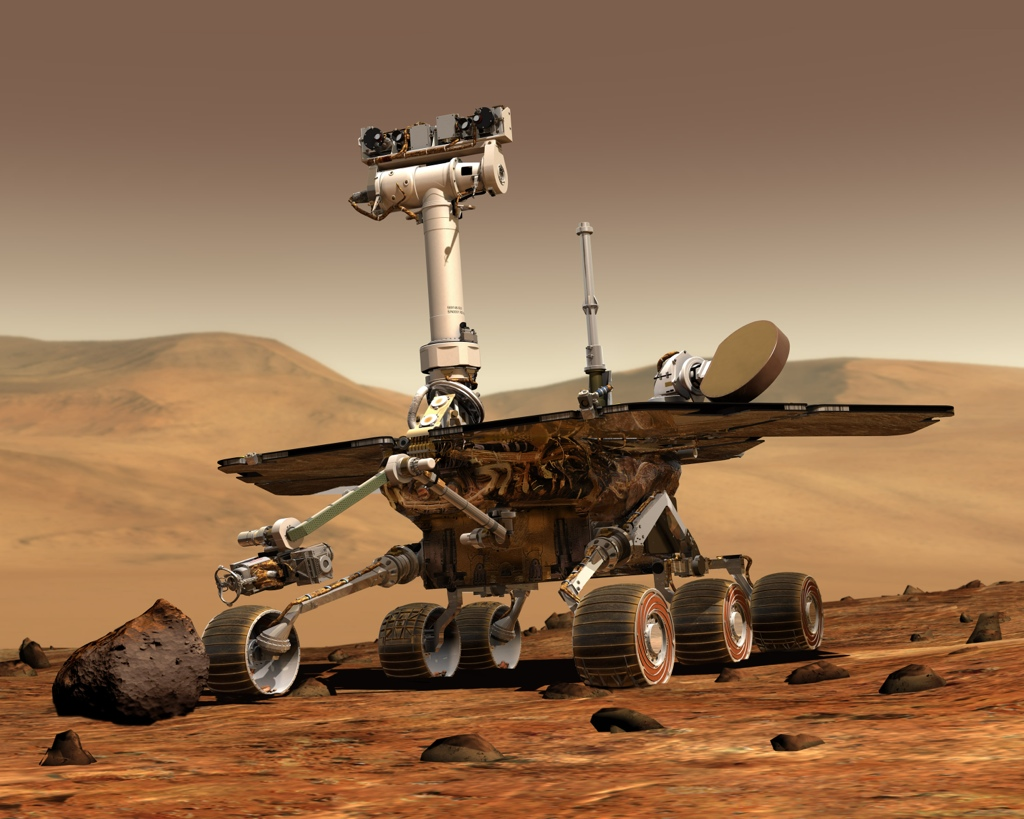
\includegraphics[width=6cm]{kapitel3/nasa_rover}
%     \caption{Ein Nasa Rover}
%     \label{Kap2:NasaRover}
% \end{figure}

% Man kann sich auch selbst ein Makro für das Einfügen von Bildern schreiben:

% \bild{kapitel3/modell_point_to_point}{6cm}{Point to Point}

% \begin{sidewaysfigure}
%     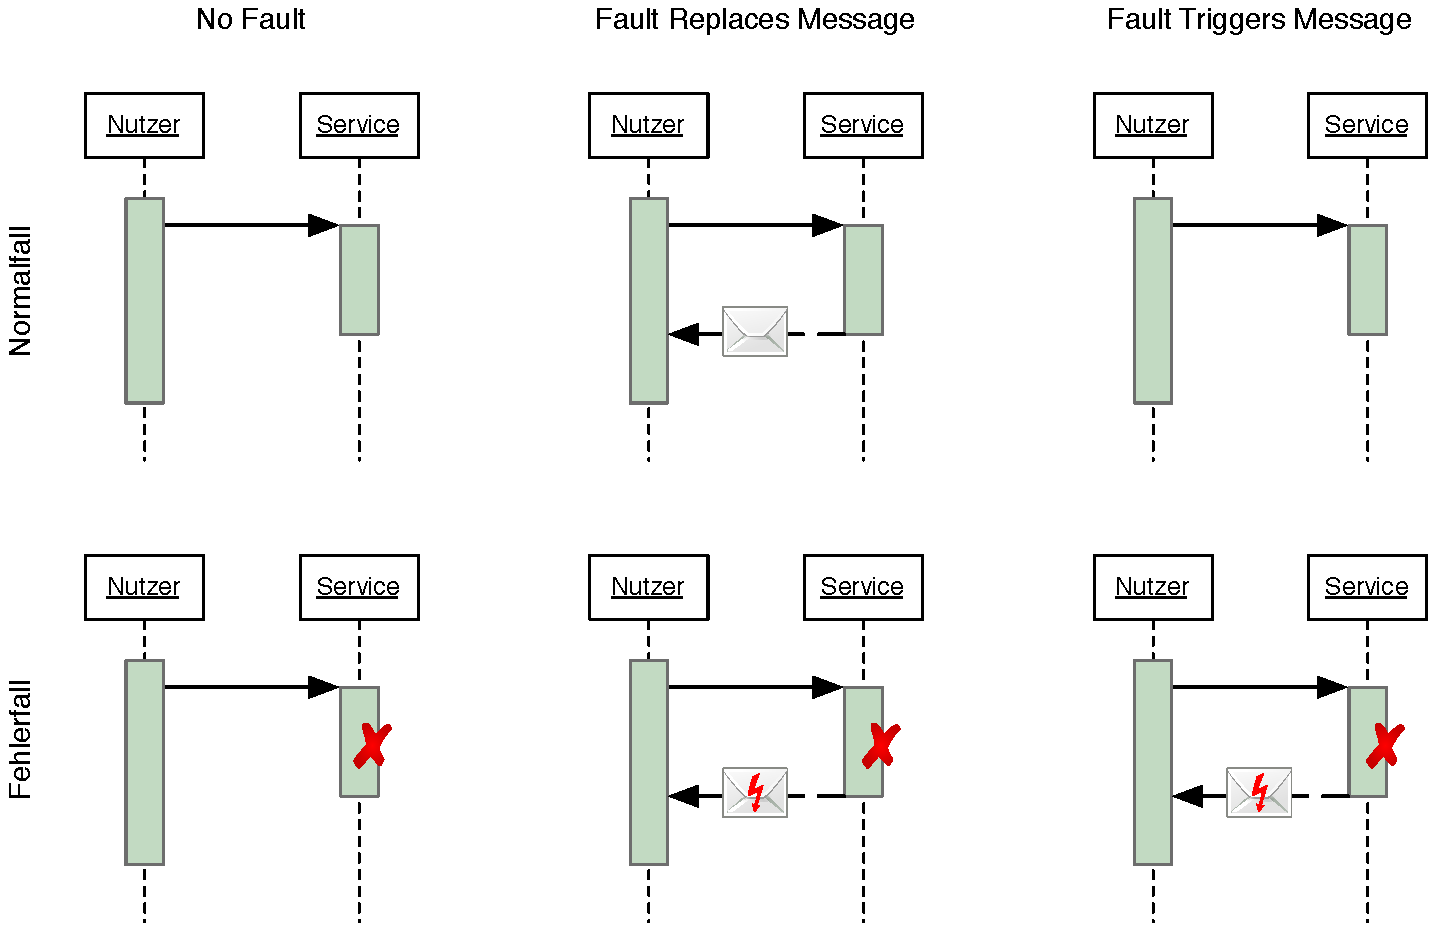
\includegraphics[width=22cm]{kapitel3/ws-wsdl20-fehler}
%     \caption{Sehr große Grafiken kann man drehen, damit sie auf die Seite passen}
%     \label{Kap2:wsdl-fehler}
% \end{sidewaysfigure}

% \clearpage % Alle Bilder, die bisher kamen ausgeben


% \section{Formelsatz}

% Eine Formel gefällig? Mitten im Text $a_2 = \sqrt{x^3}$ oder als eigener Absatz (siehe Formel~\ref{Formel}):

% \begin{equation}
%     \begin{bmatrix}
%         1 & 4 & 2  \\
%         4 & 0 & -3
%     \end{bmatrix}
%     \cdot
%     \begin{bmatrix}
%         1  & 1 & 0 \\
%         -2 & 3 & 5 \\
%         0  & 1 & 4
%     \end{bmatrix}
%     {=}
%     \begin{bmatrix}
%         -7 & 15 & 28  \\
%         4  & 1  & -12
%     \end{bmatrix}
%     \label{Formel}
% \end{equation}


% \section{Sourcecode}

% Man kann mit Latex auch ganz toll Sourcecode in den Text aufnehmen.

% \subsection{Aus einer Datei}

% \lstinputlisting[firstline=2,language=Java,caption={Crypter-Interface},label=lst:CrypterInterface]{\srcloc/Crypter.java}


% \subsection{Inline}

% \begin{lstlisting}[language=Java,caption=Methode checkKey()]
%     /**
%      * Testet den Schlüssel auf Korrektheit: Er muss mindestens die Länge 1
%      * haben und darf nur Zeichen von A-Z enthalten.
%      *
%      * @param key zu testender Schlüssel
%      * @throws CrypterException wenn der Schlüssel nicht OK ist.
%      */
%     protected void checkKey(Key key) throws CrypterException {

%         // Passt die Länge?
%         if (key.getKey().length == 0) {
%             throw new CrypterException("Der Schlüssel muss mindestens " +
%                     "ein Zeichen lang sein");
%         }

%         checkCharacters(key.getKey(), ALPHABET);
%     }
% \end{lstlisting}


% \section{Anforderungen}

% Anforderungen im Format des Volere"=Templates (Snowcards) \autocite{Volere} können per Makro eingefügt werden. Das Label wird automatisch mit der Nummer erstellt, d.\,h. Sie können auf die Tabelle mit dieser referenzieren (siehe \autoref{F52}).

% \snowcard % Snowcard einbinden (Anpassungen in titelblatt.tex)
% {F52} % Nummer des Requirements
% {F} % Art
% {Hoch} % Priorität
% {User Authentifizierung} % Titel
% {Interview mit Abteilungsleiter} % Herkunft (Optional)
% {F12} % Konflikte (Optional)
% {Der Benutzer ist in der Lage sich über seinen
%     Benutzernamen und sein Passwort am System anzumelden} % Beschreibung
% {Ein Benutzer kann sich mit seinem firmenweiten Benutzernamen und
%     Passwort über die Anmeldemaske anmelden und hat Zugriff auf die
%     Funktionen des Systems} % Fit-Kriterium (Optional)
% {Benutzerhandbuch des Altsystems} % Material (Optional)

% Ebenso können Sie nicht"=funktionale Anforderungen mit Hilfe von Quality Attribute Scenarios (vgl. \autoref{NF11}) darstellen. Zu Details siehe \autocite{Barbacci2003}.

% \qas % Quality-Attribute Scenario einbinden (Anpassungen in titelblatt.tex)
% {NF11} % Nummer des Requirements
% {Hoch} % Priotität
% {Performance des Jahresabschlusses} % Titel
% {Endbenutzer} % Quelle
% {Startet einen Jahresabschluss} % Stimulus
% {Buchhaltungssystem} % Artefakt
% {Das System befindet sich im normalen Betriebszustand} % Umgebung
% {Jahresabschluss ist durchgeführt und kann als PDF abgerufen werden} % Antwort
% {10 Minuten} % Antwort-Maß

% Die Abgrenzung von funktionalen und nicht-funktionalen Anforderungen ist nicht immer einfach und bereitet manchen Studierenden Probleme. Als Hilfestellung kann die von der ISO25010 \autocite{ISO25010} zur Verfügung gestellte Liste dienen, siehe \autoref{kapitel3/iso25010}.

% \bild{kapitel3/iso25010}{14cm}{Qualitätsmodell für Software-Produkte nach ISO25010}

% \citeauthor{Bass2003} listen in \autocite{Bass2003} eine ähnliche Liste von Kategorien für nicht-funktionalen Anforderungen auf, die ebenfalls als Richtschnur dienen kann. Diese sind:

% \begin{itemize}
%     \item \textit{Verfügbarkeit} \textit{(availability)} -- umfasst Zuverlässigkeit (reliability), Robustheit (robustness), Fehlertoleranz (fault tolerance) und Skalierbarkeit (scalability)
%     \item \textit{Anpassbarkeit} \textit{(modifiability)}, umfasst Wartbarkeit (maintainability), Verständlichkeit (understandability) und Portabilität (portability).
%     \item \textit{Performanz} \textit{(performance)}
%     \item \textit{Sicherheit} \textit{(security)}
%     \item \textit{Testbarkeit} \textit{(testability)}
%     \item \textit{Bedienbarkeit} \textit{(usability)}
% \end{itemize}
